\mychapter{Variações de exames com QM+QT para o Moodle} \label{ch:examesQM_QT_Moodle}

Neste capítulo, será apresentado um recurso interessante do MCTest que permite exportar as variações de um exame para arquivos nos formatos Aiken e XML, que podem ser utilizados pelo Moodle para criar um banco de questões. Será utilizado um exemplo de questão da área do círculo apresentada no Capítulo \ref{ch:examesQM_QT} -- \nameref{ch:examesQM_QT}, bem como a criação de novas questões para exemplificar melhor o processo. O artigo de \citeonline{2021:Zampirolli.Batista.ea*1} detalha este recurso, e neste capítulo é resumido todo o processo.

Embora o Moodle suporte a criação de questões parametrizadas, que utilizam valores curinga, essas questões têm limitações em relação às funções disponibilizadas pela linguagem PHP. Utilizar o MCTest para criar o banco de questões é vantajoso porque suporta muito mais variações de questões. É possível, por exemplo, criar um exame contendo QMs e QTs, com respostas exatas. Em seguida, é configurado o exame para gerar variações, salvando com um destes formatos Aiken ou XML. É possível então importar esses arquivos para o banco de questões no Moodle e criar uma atividade, incluindo as questões recém-importadas. Dessa forma, é possível criar atividades muito mais parametrizadas do que as suportadas pelo Moodle utilizando os curingas.

Assim, apesar dos recursos disponíveis no Moodle, ele ainda apresenta limitações na criação de questões. Neste capítulo, será abordado como tentar contornar essas restrições para criar avaliações com diversas variações.

\section{Criando exames e exportando arquivos Aiken e XML}

Será criado um exame com três QMs paramétricas, cada uma contendo quatro alternativas, e uma QT com resposta exata. A primeira questão abordará a área do círculo, conforme apresentado no segundo exemplo da Seção \ref{sec:QMparametrica} -- \nameref{sec:QMparametrica}. As outras três questões serão definidas nas seções subsequentes.

\subsection{QM -- equação de primeiro grau -- idade}

O Código \ref{lst:questaoQM_EquacaoIdade} apresenta um algoritmo que soluciona o problema de encontrar as idades de duas pessoas, dada a soma e a diferença entre elas. O método \verb|calcular_idades| recebe como parâmetros esses dois valores e utiliza equações matemáticas para determinar as idades da pessoa e do irmão. As idades são retornadas como uma \textit{string} no formato ``x e y'', em que x e y são as idades da pessoa e do irmão, respectivamente. Caso as idades não sejam números inteiros positivos, o método retorna uma \textit{string} vazia.

O programa utiliza o método \verb|random.sample| para gerar aleatoriamente pares de valores de soma e diferença no intervalo de 2 a 29. Para cada par de valores gerado, o programa chama o método \verb|calcular_idades| e armazena as respostas válidas em uma lista. A alternativa correta da questão, apresentada na linha 36, considera os dados do enunciado e utiliza o método \verb|calcular_idades| para determinar as idades dos irmãos apresentados na Figura \ref{fig:cap09_questaoQM_EquacaoIdadePDFb}. Esta resposta, \verb|respostas[3]|, deve ser incluída na primeira alternativa (correta) do formulário da questão. As demais, encontradas nos elementos de índice 0, 1 e 2 da lista \verb|respostas|, devem ser inseridas nas demais alternativas (erradas). Se desejar gerar uma questão com um maior número de alternativas, por exemplo, 10, basta modificar a linha com o comando \verb|while| para ser menor que 10, e a alternativa correta estará no elemento 9 da lista \verb|respostas|.

\begin{listing}[!ht]
\begin{myboxCode}{corCodigo}{\textbf{Questão: }}\vspace{3mm}
\hrule
\begin{minted}[xleftmargin=20pt,linenos=true]{python}
Uma pessoa tem x anos e seu irmão tem y anos. Se a diferença entre suas idades é 
de [[code:diferenca]] anos, e a soma das idades é [[code:soma]], determine as 
idades da pessoa e do irmão, respectivamente. 

[[def: 
import random

def calcular_idades(soma, diferenca):
  """Calcula idades, dados soma e diferença.
  x + y = soma e x - y = diferenca ==> 2x = (soma + diferenca)"""

  # Calcular a idade da pessoa
  x = (soma + diferenca) / 2

  # Calcular a idade do irmão
  y = soma - x

  if not x%1 and x>0 and y>0: # somente inteiros positivos
    return f"{x:2.0f} e {y:2.0f}"
  else:
    return ""

# Lista de respostas
respostas = []

# Gerar 4 equações de reta aleatórias
while len(respostas) < 4:
  # Gerar 2 valores aleatórios
  soma, diferenca = random.sample(range(2, 30), 2)
  r = calcular_idades(soma, diferenca)
  if not r: # somente inteiros positivos
    continue
  if r not in respostas: # respostas distintas
    respostas.append(r)
    
# [[code:respostas[3]]] # última será a correta
]]
\end{minted}
\end{myboxCode}
\caption{Exemplo de QM paramétrica para calcular as idades dos irmãos.}
\label{lst:questaoQM_EquacaoIdade}
\end{listing}

\begin{figure}[!ht]
  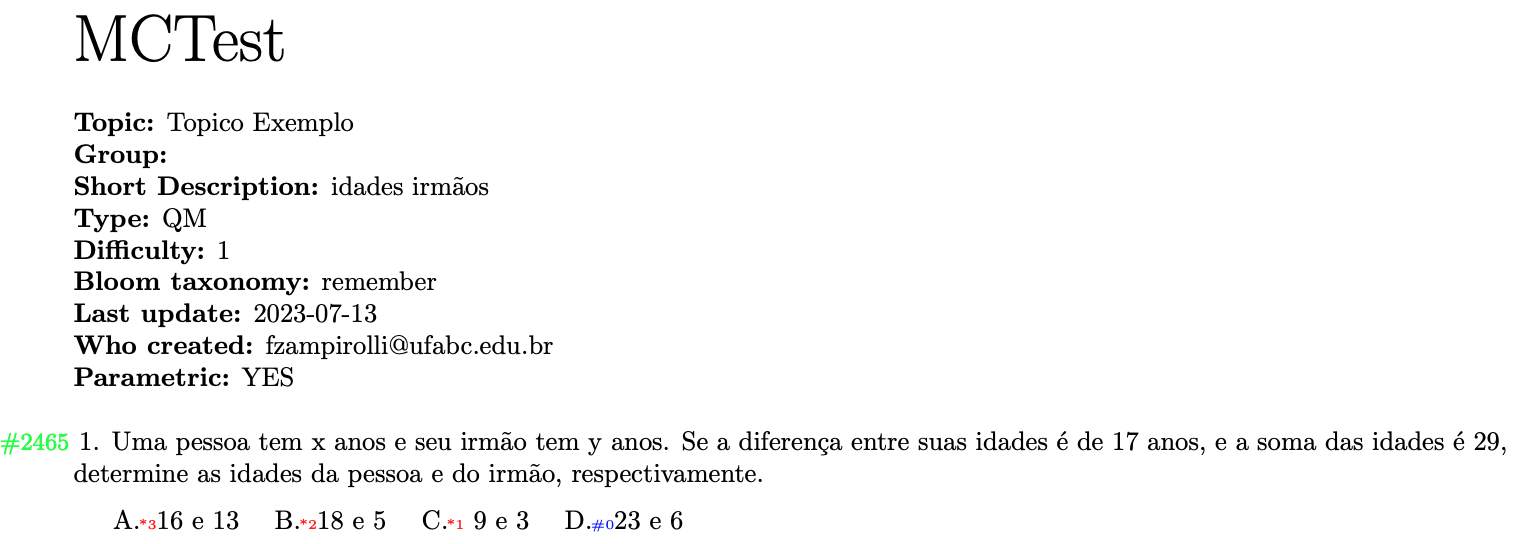
\includegraphics[width=0.9\textwidth]{cap09_questaoQM_EquacaoIdadePDF.png}
  \caption{Recorte do PDF gerado para a questão das idades dos irmãos, referente ao Código \ref{lst:questaoQM_EquacaoIdade}.}
  \label{fig:cap09_questaoQM_EquacaoIdadePDFb}
\end{figure}

\subsection{QM -- equação da reta}

O Código \ref{lst:questaoQM_EquacaoReta} implementa um algoritmo para gerar quatro equações de reta aleatórias a partir de pontos com coordenadas inteiras entre 1 e 9. O método \verb|equacao_reta| é utilizado para calcular a equação da reta que passa pelos dois pontos fornecidos. Para evitar duplicatas, o código verifica se a equação já está na lista de respostas antes de adicioná-la. Caso uma reta vertical seja gerada, ela é ignorada. A última alternativa da questão na linha 26 considera os dois pontos fornecidos no enunciado, apresentado na Figura \ref{fig:cap09_questaoQM_EquacaoRetaPDF}.

\begin{listing}[!ht]
\begin{myboxCode}{corCodigo}{\textbf{Questão: }}\vspace{3mm}
\hrule
\begin{minted}[xleftmargin=20pt,linenos=true]{python}
Qual é a equação da reta que passa pelos pontos ([[code:x1]], [[code:y1]]) e 
([[code:x2]], [[code:y2]])?

[[def: 
import random

def equacao_reta(x1, y1, x2, y2):
  """Calcula a equação da reta que passa pelos pontos (x1, y1) e (x2, y2)"""
  m = (y2 - y1) / (x2 - x1)
  b = y1 - m * x1
  return f"y = {m:.2f}x + {b:.2f}"

# Lista de respostas
respostas = []

# Gerar 4 equações de reta aleatórias e distintas
while len(respostas) < 4:
  x1,y1,x2,y2 = random.sample(range(1,10), 4) # Gerar 2 pontos aleatórios
  if x1 == x2: # A reta é vertical: não é possível calcular a inclinação m
    continue

  equacao = equacao_reta(x1, y1, x2, y2)
  if equacao not in respostas:
      respostas.append(equacao)
        
# [[code:respostas[3]]] # última será a correta
]]
\end{minted}
\end{myboxCode}
\caption{Exemplo de QM paramétrica para calcular a equação da reta.}
\label{lst:questaoQM_EquacaoReta}
\end{listing}

\begin{figure}[!ht]
  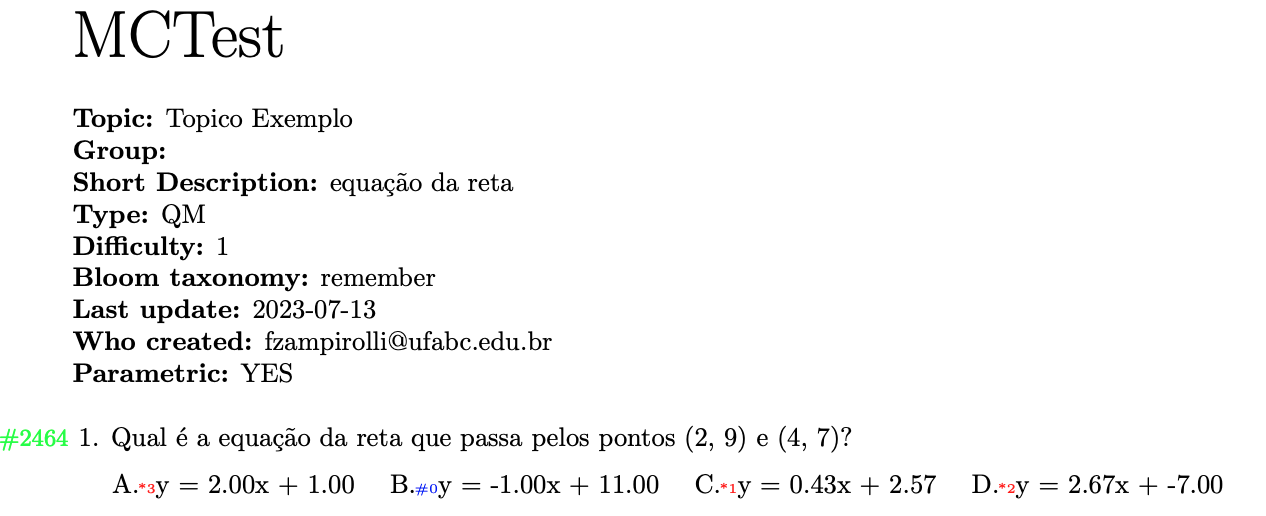
\includegraphics[width=0.9\textwidth]{cap09_questaoQM_EquacaoRetaPDF.png}
  \caption{Recorte do PDF gerado para a questão da equação da reta definida no Código \ref{lst:questaoQM_EquacaoReta}.}
  \label{fig:cap09_questaoQM_EquacaoRetaPDF}
\end{figure}

\subsection{QT com resposta exata -- ordena parte do vetor}

Na Seção \ref{sec:questoesQM_QT} -- \nameref{sec:questoesQM_QT}, foi apresentado o Código \ref{lst:questaoQT_exata}, que descreve como criar uma QT com resposta exata. Nesta seção, será apresentado um exemplo prático deste recurso, por meio da adaptação dos Códigos \ref{lst:questaoQT_EP_1_parte1} e \ref{lst:questaoQT_EP_1_parte1} de questão paramétrica integrada ao VPL.

Os Códigos \ref{lst:questaoQT_Exata_1_parte1} e \ref{lst:questaoQT_Exata_1_parte2} implementam uma questão paramétrica exata, utilizando o método \verb|ordena_parte_vetor|. Esse método recebe como entrada um vetor de números inteiros, um índice de início e um índice de fim, e ordena apenas uma parte do vetor, delimitada pelos índices de início e fim.

O método utiliza um algoritmo de ordenação por seleção simples, que percorre o trecho do vetor a ser ordenado e, em cada iteração, seleciona o menor elemento da parte não ordenada e o coloca em sua posição correta na parte ordenada. Esse algoritmo é implementado por meio de dois laços aninhados: o primeiro percorre os elementos da parte do vetor a ser ordenada, enquanto o segundo percorre os elementos ainda não ordenados. A cada iteração do segundo laço, é verificado se o elemento atual é menor do que o elemento selecionado pelo primeiro laço. Se for o caso, os elementos são trocados de posição.
%
O método retorna o vetor ordenado, e a ordenação é realizada \textit{in-place}, ou seja, o vetor original é modificado diretamente pelo método. A Figura \ref{fig:cap09_questaoQT_Exata_PDF} apresenta um exemplo para esta questão.

A questão apresentada nos Códigos \ref{lst:questaoQT_Exata_1_parte1} e \ref{lst:questaoQT_Exata_1_parte2} já está preparada para ser aplicada em atividades VPL, seguindo os Códigos \ref{lst:questaoQT_EP_1_parte1} e \ref{lst:questaoQT_EP_1_parte1}. No entanto, a parte crítica é a formatação da questão, limitada pelo Moodle, como serão apresentadas nas próximas seções.

Esta questão de ordenar vetor é um exemplo típico que não pode ser implementado no Moodle utilizando os valores curinga. Isso ilustra que para questões mais complexas, o MCTest é uma ferramenta adequada para criar um banco de questões e exportá-lo para o Moodle.


\begin{listing}[!ht]
\begin{myboxCode}{corCodigo}{\textbf{Questão: }}\vspace{3mm}
\hrule
\begin{minted}[xleftmargin=20pt,linenos=true]{python}
Dado um vetor de inteiros de tamanho \( n = [[code:n]]\), ordenar o trecho do 
vetor que começa no índice \( inicio = [[code:inicio]] \) e termina no índice 
\( fim = [[code:fim]]\). Onde, \( 0 < inicio < fim < n \), ou seja, o trecho a 
ser ordenado está entre início (inclusive) e fim (inclusive). Vale ressaltar 
que os índices do vetor começam em 0 e terminam em \( n-1\). 

Considere esta entrada:} 
[[code:caso0_inp]]

%%{[[code:caso0_out]]}%%
\end{minted}
\end{myboxCode}
\caption{Exemplo de questão paramétrica exata -- Parte 1: Descrição de questão.}
\label{lst:questaoQT_Exata_1_parte1}
\end{listing}

\begin{listing}[!h]
\begin{myboxCode}{corCodigo}{\textbf{Questão: }}\vspace{3mm}
\hrule
\begin{minted}[xleftmargin=20pt,linenos=true]{python}
[[def: 
import json, numpy as np

# Passo 1: Criar os parâmetros do enunciado da questão
n = np.random.randint(20,40)
inicio = np.random.randint(2,n//2-2)
fim = np.random.randint(n//2+2,n-2)
    
# Passo 2: Criar os casos de teste
inp_list, out_list = [], []  # Listas vazias para armazenar os casos de teste
casos_teste = 1  # Número de casos de teste desejado

def ordena_parte_vetor(vetor,inicio,fim):        
    """ Ordenação da parte do vetor entre inicio e fim"""
    for i in range(inicio, fim+1):
        for j in range(i+1, fim+1):
            if vetor[i] > vetor[j]:
                vetor[i], vetor[j] = vetor[j], vetor[i]
    # Retorno do vetor ordenado
    return vetor
    
# Para cada caso de teste:
for i in range(casos_teste):    

    #>>>> begin - casos de teste
    # Gerar valores aleatórios entre 0 e 9 para o vetor 
    v = np.random.randint(10, size=n) 

    # Criar a entrada do caso de teste como uma string
    inp = ' '.join(str(i) for i in v) + '\n'

    # Calcular o vetor de saída
    out = ' '.join(str(i) for i in ordena_parte_vetor(v,inicio,fim)) # + '\n'
    #<<<< end - casos de teste

    # Adicionar a entrada e saída do caso de teste às listas
    inp_list.append(inp), out_list.append(out)

# Passo 3: Criar o dicionário com os casos de teste
cases = {}
cases['input']  = np.array(inp_list).tolist()
cases['output'] = np.array(out_list).tolist()

# Passo 4: Mostrar um exemplo no enunciado da questão
caso0_inp, caso0_out = cases['input'][0], cases['output'][0]
]]
\end{minted}
\end{myboxCode}
\caption{Exemplo de questão paramétrica exata -- Parte 2: Bloco de código.}
\label{lst:questaoQT_Exata_1_parte2}
\end{listing}

\begin{figure}[!ht]
  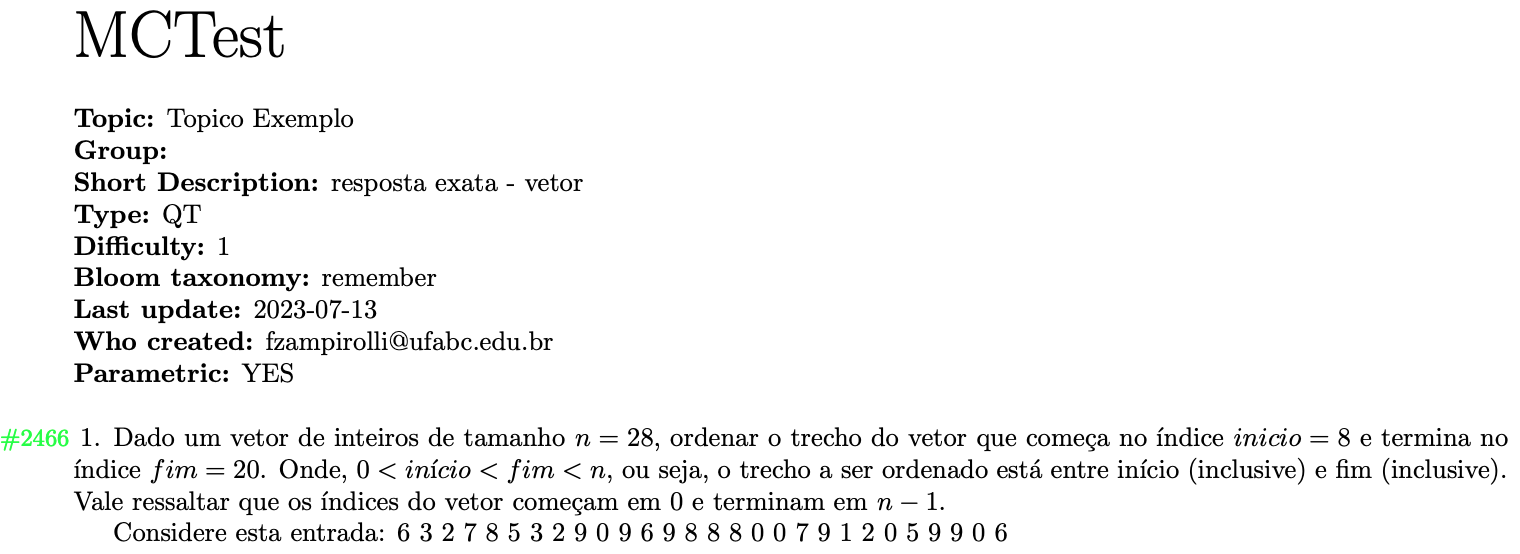
\includegraphics[width=0.9\textwidth]{cap09_questaoQT_Exata_PDF.png}
  \caption{Recorte do PDF gerado para a questão com resposta exata definida pelos Códigos \ref{lst:questaoQT_Exata_1_parte1} e \ref{lst:questaoQT_Exata_1_parte2}.}
  \label{fig:cap09_questaoQT_Exata_PDF}
\end{figure}

\ 
\newpage

\

\begin{mybox}{corEdicao2}{\textbf{Destaque:\\\vspace{-3mm}\hrule\vspace{3mm}}}
  \begin{enumerate}
    \item No final da linha 33 do Código \ref{lst:questaoQT_Exata_1_parte2}, foi necessário adicionar um comentário para assegurar uma formatação adequada da questão no Moodle. Essa informação está presente no enunciado da questão, na linha 10 do Código \ref{lst:questaoQT_Exata_1_parte1}, com o intuito de armazenar a resposta correta da questão.
    \item As mudanças de linha são obrigatórias a cada entrada/saída nas questões com integração VPL, conforme apresentado no Capítulo \ref{ch:questoesCodigoMCTest} -- \nameref{ch:questoesCodigoMCTest} e também serão destacadas no próximo capítulo.
  \end{enumerate}  
\end{mybox}

\subsection{QT para a integração MCTest+Moodle+CodeRunner}\label{sec:questoesQM_QT_CodeRunner}

A nova versão do MCTest 5.3 permite gerar XML para questões QT, compatível com o \textit{plugin} \href{https://moodle.org/plugins/qtype_coderunner}{CodeRunner}. Para utilizar essa funcionalidade, configure a questão como nos exemplos dos Códigos \ref{lst:questaoQT_Exata_1_parte1} e \ref{lst:questaoQT_Exata_1_parte2}.

Após a linha 42 do Código \ref{lst:questaoQT_Exata_1_parte2}, adicione a seguinte linha para inserir a solução da questão em código:

\verb|cases['answer'] = ['''sua solução''']|

O método \verb|createFileDB_xml()| contido no arquivo \verb|UtilsLatex| na pasta de exames no \href{https://github.com/fzampirolli/mctest/blob/master/exam/UtilsLatex.py}{github.com/fzampirolli/mctest} pode ser consultado para obter mais detalhes sobre a geração do XML. Vale notar que o texto da questão no formato \LaTeX{} é convertido de forma automática para o formato HTML utilizando o pacote \href{https://pandoc.org}{pandoc}; veja o método \verb|latex_to_html()| neste mesmo arquivo \verb|UtilsLatex|.

\subsection{Criando exame e exportando as variações}

Com as questões definidas anteriormente, é possível agora criar um exame seguindo as instruções apresentadas no Capítulo \ref{ch:exames} -- \nameref{ch:exames}, e exportar as variações necessárias.

Após a criação do exame, é possível selecionar as quatro questões apresentadas na Figura \ref{fig:cap09_exameVariacoes_questoes}. Os detalhes do exame são apresentados na Figura \ref{fig:cap09_exameVariacoes_detalhes}. É importante notar que foi decidido criar somente cinco variações.

\begin{figure}[!ht]
\centering
  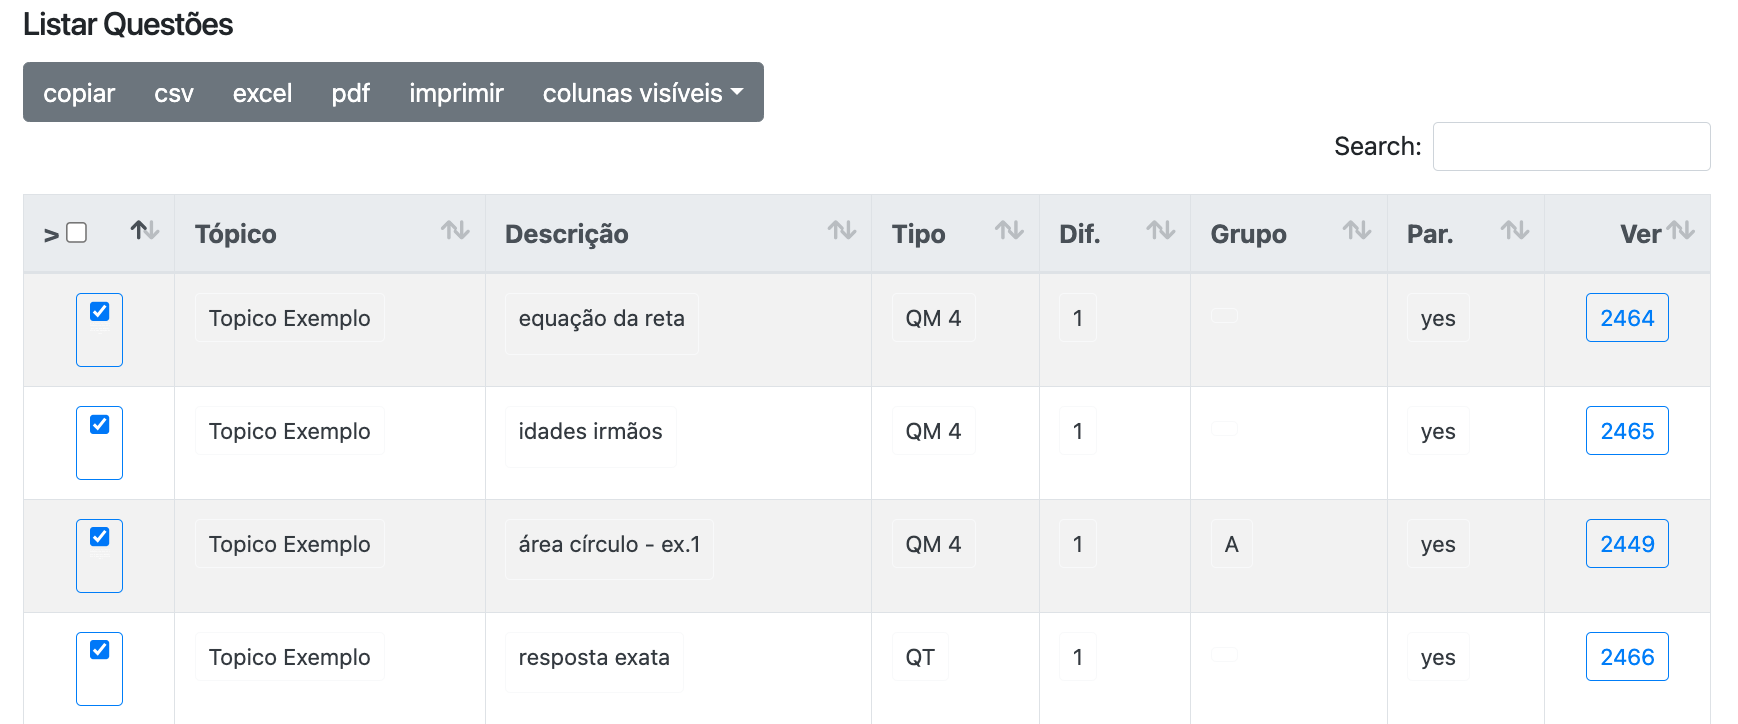
\includegraphics[width=0.9\textwidth]{cap09_exameVariacoes_questoes.png}
  \caption{Recorte da tela do exame com as quatro questões marcadas.}
  \label{fig:cap09_exameVariacoes_questoes}
\end{figure}

\begin{figure}[!ht]
\centering
  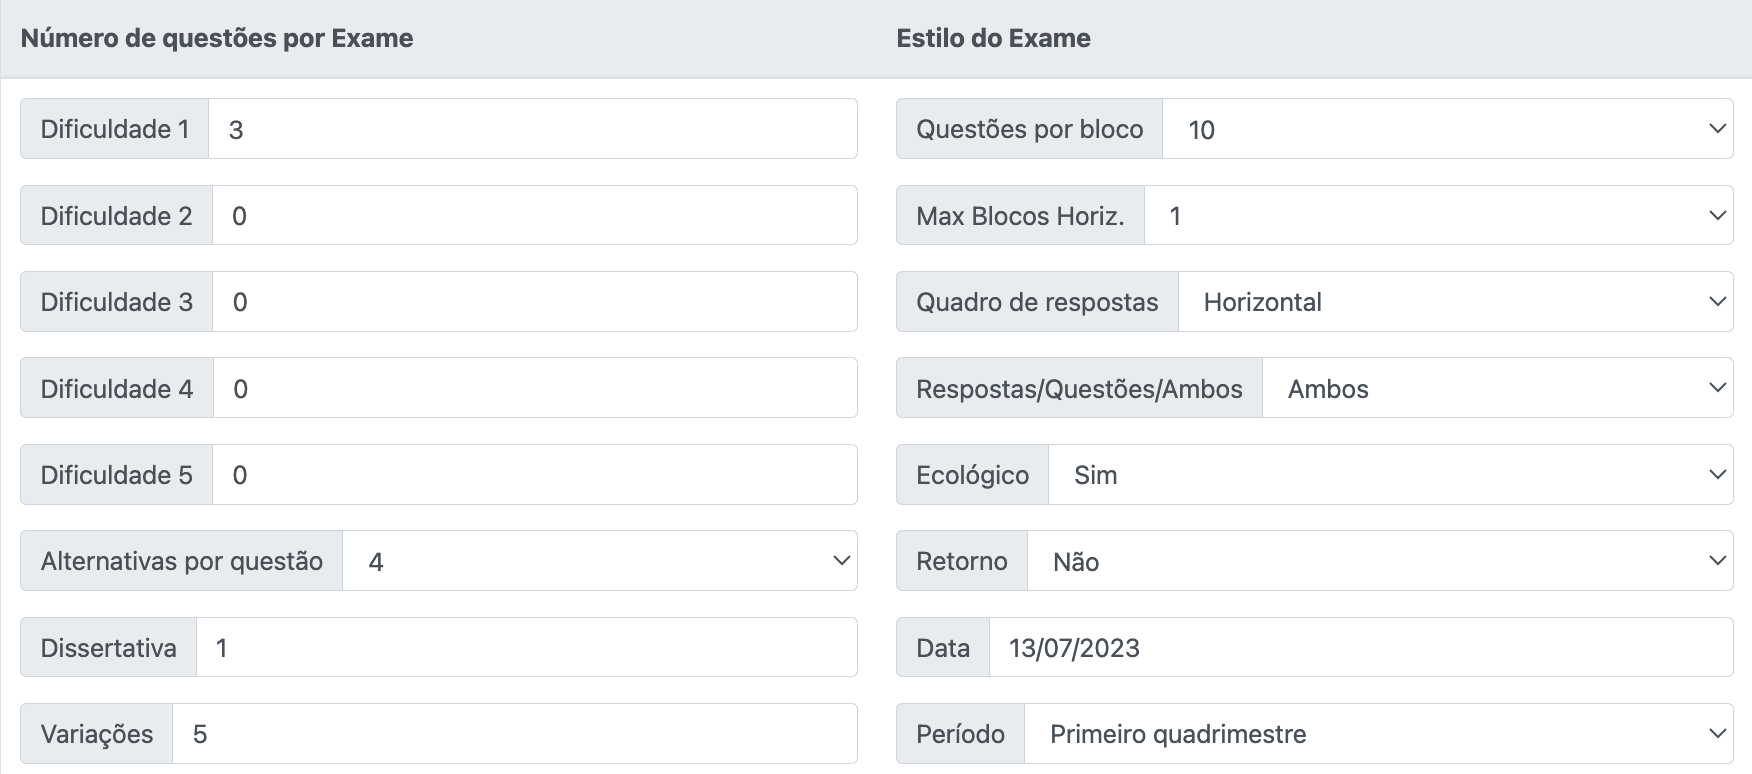
\includegraphics[width=0.9\textwidth]{cap09_exameVariacoes_detalhes.png}
  \caption{Recorte da tela do exame com os detalhes da configuração.}
  \label{fig:cap09_exameVariacoes_detalhes}
\end{figure}

Para prosseguir com a criação das variações, é necessário selecionar as opções ``Aiken'' e ``XML'', conforme ilustrado na Figura \ref{fig:cap09_exameVariacoes_variacoes}, e em seguida clicar em ``Criar-Variações''. O professor receberá um e-mail contendo dois anexos: um no formato Aiken (TXT) e outro no formato XML, como mostrado na Figura \ref{fig:cap09_xameVariacoes_variacoes_email}. No caso deste exame com ID 480 recém-criado, os arquivos recebidos serão:\\

\begin{myboxCode}{corCSV}{\textbf{Arquivos em formatos Aiken (TXT) e XML}}\vspace{3mm}
\hrule
{\footnotesize
\begin{verbatim}
report_Exam_480_variations_DB_aiken.txt
report_Exam_480_variations_DB.xml
\end{verbatim}
}
\end{myboxCode}

\begin{figure}[!ht]
\centering
  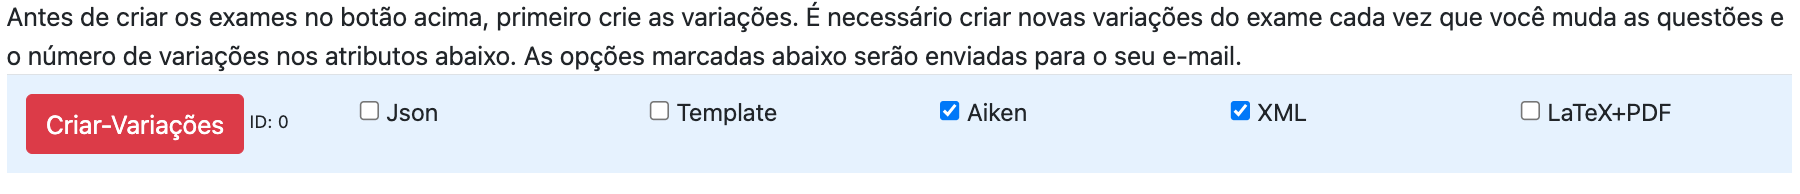
\includegraphics[width=0.9\textwidth]{cap09_exameVariacoes_variacoes.png}
  \caption{Recorte da tela do exame com os detalhes da configuração.}
  \label{fig:cap09_exameVariacoes_variacoes}
\end{figure}

\begin{figure}[!ht]
\centering
  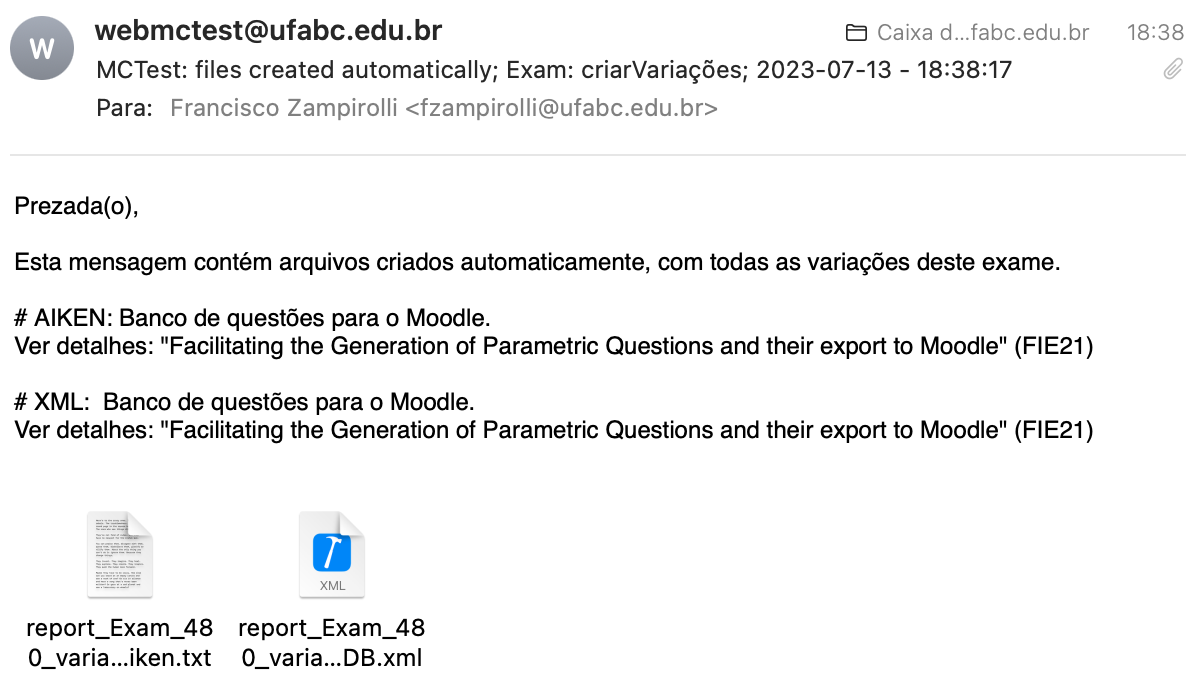
\includegraphics[width=0.9\textwidth]{cap09_exameVariacoes_variacoes_email.png}
  \caption{Recorte do e-mail recebido após clicar em ``Criar-Variações''.}
  \label{fig:cap09_xameVariacoes_variacoes_email}
\end{figure}

\subsubsection{Detalhando o arquivo no formato Aiken}

A seguir, são apresentadas as três QMs da primeira variação. Vale ressaltar que, na Figura \ref{fig:cap09_exameVariacoes_detalhes}, foram solicitadas cinco variações no formato Aiken, geradas pelo MCTest. No entanto, antes de importá-las no Moodle, é necessário remover os comentários adicionados pelo MCTest apenas para controle. Em versões de produção do MCTest, esses comentários podem ser facilmente removidos. Além disso, um aspecto desagradável deste formato é que não é possível importar questões com apenas resposta exata.

\begin{myboxCode}{corCSV}{\textbf{Conteúdo do arquivo \texttt{*\_aiken.txt}, variação 0 e questão 1.}}\vspace{3mm}
\hrule
\begin{verbatim}
############# variation ########## 0

#c:1 #id:2465 #topic:Topico Exemplo #type:QM #diff:1

Uma pessoa tem x anos e seu irmão tem y anos. Se a diferença entre suas idades é de 
2 anos, e a soma das idades é 28, determine as idades da pessoa e do irmão,
respectivamente. 
A) 15 e 13
B) 20 e  1
C) 11 e  2
D) 18 e  1
ANSWER: A
...
\end{verbatim}
\end{myboxCode}

\begin{myboxCode}{corCSV}{\textbf{Conteúdo do arquivo \texttt{*\_aiken.txt}, variação 0 e questão 2.}}\vspace{3mm}
\hrule
\begin{verbatim}
...
#c:2 #id:2449 #topic:Topico Exemplo #type:QM #diff:1

Qual é a área do círculo de raio \( 25 \)?
% comentário em LaTex. Observe que a variável raio1, após "code:" 
% foi definida na linha 18 abaixo
A) 2827.43
B) 3019.07
C) 1809.56
D) 1963.50
ANSWER: D

#c:3 #id:2464 #topic:Topico Exemplo #type:QM #diff:1

Qual é a equação da reta que passa pelos pontos (2, 7) e (8, 6)?
A) y = 1.00x + -2.00
B) y = -0.17x + 7.33
C) y = 2.00x + 1.00
D) y = 1.00x + 4.00
ANSWER: B
\end{verbatim}
\end{myboxCode}

\subsubsection{Detalhando o arquivo no formato XML para QM}

A seguir é detalhado o arquivo no formato XML que contém a primeira QM da primeira variação. Diferentemente do formato Aiken, os comentários iniciados com o símbolo ``\#'' neste formato XML não precisam ser removidos. No entanto, antes de importá-las no Moodle, é necessário remover os comentários em \LaTeX{} dentro de cada questão e gerar novamente o arquivo. Realizar esse processo diretamente no arquivo XML pode ser mais complexo e propenso a erros, especialmente se for necessário gerar muitas variações. Por isso, é recomendado gerar uma única variação e verificar como ela é formatada no Moodle antes de prosseguir com a geração de outras variações.

Cabe salientar que a sintaxe no formato XML é complexa e não é destinada ao consumo humano. Por isso, foi apresentada somente a primeira QM gerada a seguir.

Foi criada, no código XML a seguir, uma hierarquia de categorias para as questões com base nas suas características, tais como tipo, tópico e nível de dificuldade. Essa organização visa tornar o banco de questões mais estruturado no Moodle. Além disso, foi criada uma categoria para cada questão do MCTest, facilitando a localização das questões no Moodle.
\
No exemplo a seguir, é apresentada a hierarquia de categorias  \verb|multichoice/Topico Exemplo/diff1/área círculo - ex.1|.


% \tiny < \scriptsize < \footnotesize < \small < \normalsize < \large < \Large < \LARGE < \huge < \Huge

\begin{myboxCode}{corCSV}{\textbf{Conteúdo do arquivo \texttt{*.xml}, variação 0 e questão 1 -- categoria.}}\vspace{3mm}
\hrule
{\scriptsize
\begin{verbatim}
<?xml version="1.0" encoding="UTF-8"?>
<quiz>
    <!-- category:  #id:2449 #type:multichoice #topic:Topico Exemplo #diff:1 #descr:área círculo - ex.1  -->
    
    <question type="category">
    
        <category>
        
            <text>
            
                $course$/top/multichoice/Topico Exemplo/diff1/área círculo - ex.1
            
            </text>
            
        </category>
        
        <info format="moodle_auto_format">
        
            <text></text>
            
        </info>
        
        <idnumber></idnumber>
        
    </question>
...
\end{verbatim}
}
\end{myboxCode}



\begin{myboxCode}{corCSV}{\textbf{Conteúdo do arquivo \texttt{*.xml}, variação 0 e questão 1.}}\vspace{3mm}
  \hrule
  {\scriptsize
  \begin{verbatim}
  ...
  <!-- question:#c:2#id:2449#type:multichoice#topic:Topico Exemplo#diff:1#descr:área círculo - ex.1#var:1-->
  
            <question type="multichoice">
  
              <name>
                <text>Topico: Topico Exemplo Dificuldade: 1 </text>
              </name>
              
              <questiontext format="moodle_auto_format">
              
                  <text><![CDATA[<p> Qual é a área do círculo de raio \( 25 \)?
  % comentário em LaTex. Observe que a variável raio1, após "code:" 
  % foi definida na linha 18 abaixo
  
   <br></p>]]>
                  </text>
  
              </questiontext>
...
\end{verbatim}
}
\end{myboxCode}
            
\begin{myboxCode}{corCSV}{\textbf{Conteúdo do arquivo \texttt{*.xml}, variação 0 e questão 1.}}\vspace{3mm}
\hrule
{\scriptsize
\begin{verbatim}
...
            <generalfeedback format="moodle_auto_format">
              <text></text>
            </generalfeedback>
            
            <defaultgrade>1.0000000</defaultgrade>
            
            <penalty>0.3333333</penalty>

            <hidden>0</hidden>
            
            <idnumber></idnumber>
            
            <single>true</single>
            
            <shuffleanswers>true</shuffleanswers>
            
            <answernumbering>abc</answernumbering>
            
            <correctfeedback format="moodle_auto_format">
              <text>Sua resposta está correta.</text>
            </correctfeedback>
            
            <partiallycorrectfeedback format="moodle_auto_format">
              <text>Sua resposta está parcialmente correta.</text>
            </partiallycorrectfeedback>
            
            <incorrectfeedback format="moodle_auto_format">
              <text>Sua resposta está incorreta.</text>
            </incorrectfeedback>

            <shownumcorrect/>    
...
\end{verbatim}
}
\end{myboxCode}


\begin{myboxCode}{corCSV}{\textbf{Conteúdo do arquivo \texttt{*.xml}, variação 0 e questão 1 -- alternativas.}}\vspace{3mm}
\hrule
{\scriptsize
\begin{verbatim}
...
            <answer fraction="0" format="moodle_auto_format">
            
              <text><![CDATA[<p> 2827.43
 <br></p>]]></text>
            
              <feedback format="moodle_auto_format">
                <text></text>
              </feedback>
              
            </answer>
...
\end{verbatim}
}
\end{myboxCode}

\begin{myboxCode}{corCSV}{\textbf{Conteúdo do arquivo \texttt{*.xml}, variação 0 e questão 1 -- alternativas.}}\vspace{3mm}
\hrule
{\scriptsize
\begin{verbatim}
...
            <answer fraction="0" format="moodle_auto_format">
            
              <text><![CDATA[<p> 3019.07
 <br></p>]]></text>
 
              <feedback format="moodle_auto_format">
                <text></text>
              </feedback>
              
            </answer>
...
\end{verbatim}
}
\end{myboxCode}

\begin{myboxCode}{corCSV}{\textbf{Conteúdo do arquivo \texttt{*.xml}, variação 0 e questão 1 -- alternativas.}}\vspace{3mm}
\hrule
{\scriptsize
\begin{verbatim}
...
            <answer fraction="0" format="moodle_auto_format">
            
              <text><![CDATA[<p> 1809.56
 <br></p>]]></text>
 
              <feedback format="moodle_auto_format">
                <text></text>
              </feedback>
              
            </answer>
...
\end{verbatim}
}
\end{myboxCode}

\begin{myboxCode}{corCSV}{\textbf{Conteúdo do arquivo \texttt{*.xml}, variação 0 e questão 1 -- alternativas.}}\vspace{3mm}
\hrule
{\scriptsize
\begin{verbatim}
...
            <answer fraction="100" format="moodle_auto_format">
            
              <text><![CDATA[<p> 1963.50
 <br></p>]]></text>
 
              <feedback format="moodle_auto_format">
                <text></text>
              </feedback>
              
            </answer>
        
        </question>     
...
\end{verbatim}
}
\end{myboxCode}

\subsubsection{Detalhando o arquivo no formato XML -- questão com resposta exata}

A seguir, serão apresentados os detalhes do arquivo XML referente à questão com resposta exata. A hierarquia desta questão foi \verb|top/shortanswer/Topico Exemplo/diff1/resposta exata|. É relevante ressaltar que essa questão foi agrupada na categoria \verb|shortanswer|, diferentemente das QMs, que utilizam a categoria \verb|multichoice|. É importante lembrar que é necessário criar as questões no formato adequado no MCTest para poderem ser importadas e exibidas corretamente no Moodle, que possui sua própria formatação.

\begin{myboxCode}{corCSV}{\textbf{Conteúdo do arquivo \texttt{*.xml}, variação 0 e questão com resposta exata -- categoria.}}\vspace{3mm}
\hrule
{\scriptsize
\begin{verbatim}
...
        <!-- category:#id:2466#type:shortanswer#topic:Topico Exemplo#diff:1#descr:resposta exata - vetor-->
        <question type="category">
            <category>
                <text>
                    $course$/top/shortanswer/Topico Exemplo/diff1/resposta exata - vetor
                </text>
            </category>
            
            <info format="moodle_auto_format">
            <text></text>
            </info>
            
            <idnumber></idnumber>
        </question>
...
\end{verbatim}
}
\end{myboxCode}

\begin{myboxCode}{corCSV}{\textbf{Conteúdo do arquivo \texttt{*.xml}, variação 0 e questão com resposta exata -- questão.}}\vspace{3mm}
\hrule
{\scriptsize
\begin{verbatim}
...
<!--question:#c:4#id:2466#type:shortanswer#topic:Topico Exemplo#diff:1#descr:resposta exata - vetor#var:1-->

          <question type="shortanswer">
          
            <name>
              <text>Topico: Topico Exemplo Dificuldade: 1 </text>
            </name>
            
            <questiontext format="moodle_auto_format">
            
            <text>
            
            <![CDATA[<p> Dado um vetor de inteiros de tamanho \( n = 31\), ordenar o trecho do 
vetor que começa no índice \( inicio = 10 \) e termina no índice 
\( fim = 24\). Onde, \( 0 < inicio < fim < n \), ou seja, o trecho 
a ser ordenado está entre início (inclusive) e fim (inclusive). Vale 
ressaltar que os índices do vetor começam em 0 e terminam em \( n-1\). 
            
Considere esta entrada:
8 1 4 1 2 0 1 6 1 9 6 3 7 2 7 8 9 3 7 2 0 7 6 4 3 0 1 1 9 4 1
  
 <br></p>]]>
 
            </text>
 
            </questiontext>         
...
\end{verbatim}
}
\end{myboxCode}

\begin{myboxCode}{corCSV}{\textbf{Conteúdo do arquivo \texttt{*.xml}, variação 0 e questão com resposta exata -- resposta.}}\vspace{3mm}
\hrule
{\scriptsize
\begin{verbatim}
...

            <generalfeedback format="moodle_auto_format">
              <text></text>
            </generalfeedback>
            
            <defaultgrade>1.0000000</defaultgrade>
            
            <penalty>0.3333333</penalty>
            
            <hidden>0</hidden>
            
            <idnumber></idnumber>
            
            <single>true</single>
            
            <shuffleanswers>true</shuffleanswers>
            
            <answernumbering>abc</answernumbering>
            
            <correctfeedback format="moodle_auto_format">
            
              <text>Sua resposta está correta.</text>
              
            </correctfeedback>
            
            <partiallycorrectfeedback format="moodle_auto_format">
            
              <text>Sua resposta está parcialmente correta.</text>
              
            </partiallycorrectfeedback>
            
            <incorrectfeedback format="moodle_auto_format">
              <text>Sua resposta está incorreta.</text>
            </incorrectfeedback>
            
            <shownumcorrect/>        
            
    <answer fraction="100" format="moodle_auto_format">
    
        <text>
            8 1 4 1 2 0 1 6 1 9 0 2 2 3 3 3 4 6 6 7 7 7 7 8 9 0 1 1 9 4 1
        </text>
        
    </answer>
    
</question>

...
\end{verbatim}
}
\end{myboxCode}

\section{Importando arquivo XML no Moodle}

Como o formato Aiken apresenta algumas limitações, como a impossibilidade de criar questões com resposta exata, será apresentado a seguir um tutorial para importar e criar questionários no Moodle usando o formato XML.

Considerando a versão 4.1 do Moodle, é necessário importar o arquivo XML gerado pelo MCTest. Para fazer isso, acesse a opção ``Banco de questões'', disponível no ícone de engrenagem no canto superior direito ou no menu ``Administração'' à esquerda. Em seguida, basta escolher a opção ``Importação'', selecionar o formato XML e mover o arquivo correspondente para a área especificada. Ao clicar em ``Importar'', as 20 questões serão carregadas e poderão ser visualizadas, como ilustrado na Figura \ref{fig:cap09_exameVariacoes_QM_moodle} para uma QM e na Figura \ref{fig:cap09_exameVariacoes_exata_moodle} para uma questão com resposta exata. Na Figura \ref{fig:cap09_exameVariacoes_detalhes} foram 3 QMs, 1 QT e 5 variações ($(3+1)*5=20$).

Vale ressaltar que o uso de formatação em \LaTeX{} no Moodle apresenta muitas limitações em comparação com o PDF gerado pelo MCTest, como ilustrado na Figura \ref{fig:cap09_exameVariacoes_exata_moodle}.

\begin{figure}[!ht]
\centering
  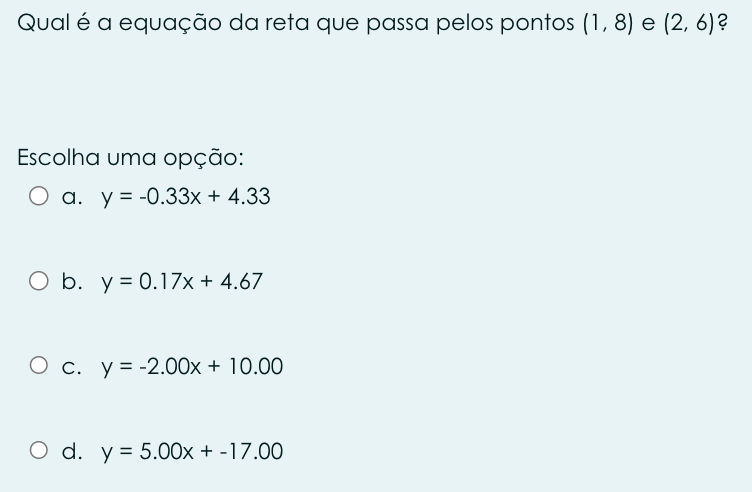
\includegraphics[width=0.9\textwidth]{cap09_exameVariacoes_QM_moodle.png}
    \caption{Exemplo de QM no Moodle.}
  \label{fig:cap09_exameVariacoes_QM_moodle}
\end{figure}

\begin{figure}
\centering
  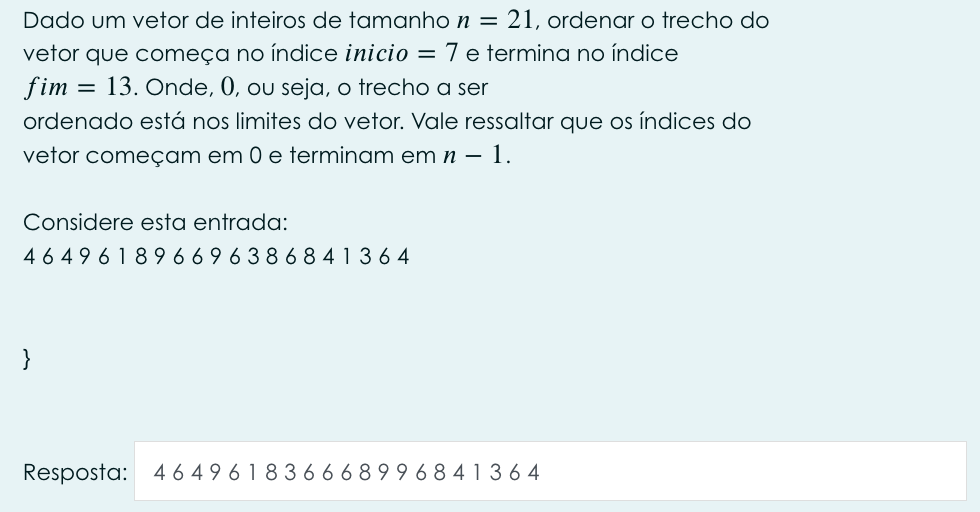
\includegraphics[width=0.9\textwidth]{cap09_exameVariacoes_exata_moodle.png}
  \caption{Exemplo da questão exata do Moodle.}
  \label{fig:cap09_exameVariacoes_exata_moodle}
\end{figure}

Em termos de comparação, observe na Figura \ref{fig:cap09_exameVariacoes_PDF_MCTest} como seria um exame em PDF gerado pelo MCTest com essas variações das 3 QMs, seguido por uma QT com resposta exata. O professor também pode corrigir esse estilo de exame digitalizando-o para corrigir as QMs. Quanto à QT, o professor pode corrigi-la manualmente, comparando a resposta exata do estudante com o gabarito gerado pelo MCTest ao escolher a opção ``Template'' antes de clicar em ``Criar-Variações''. O artigo de \citeonline{2020:Zampirolli.Batista.ea} detalha esse processo de correção automática utilizando a opção ``Template'', também resumido na Seção \ref{sec:experMCTestForms} -- \nameref{sec:experMCTestForms}.


\begin{figure}[!ht]
\centering
  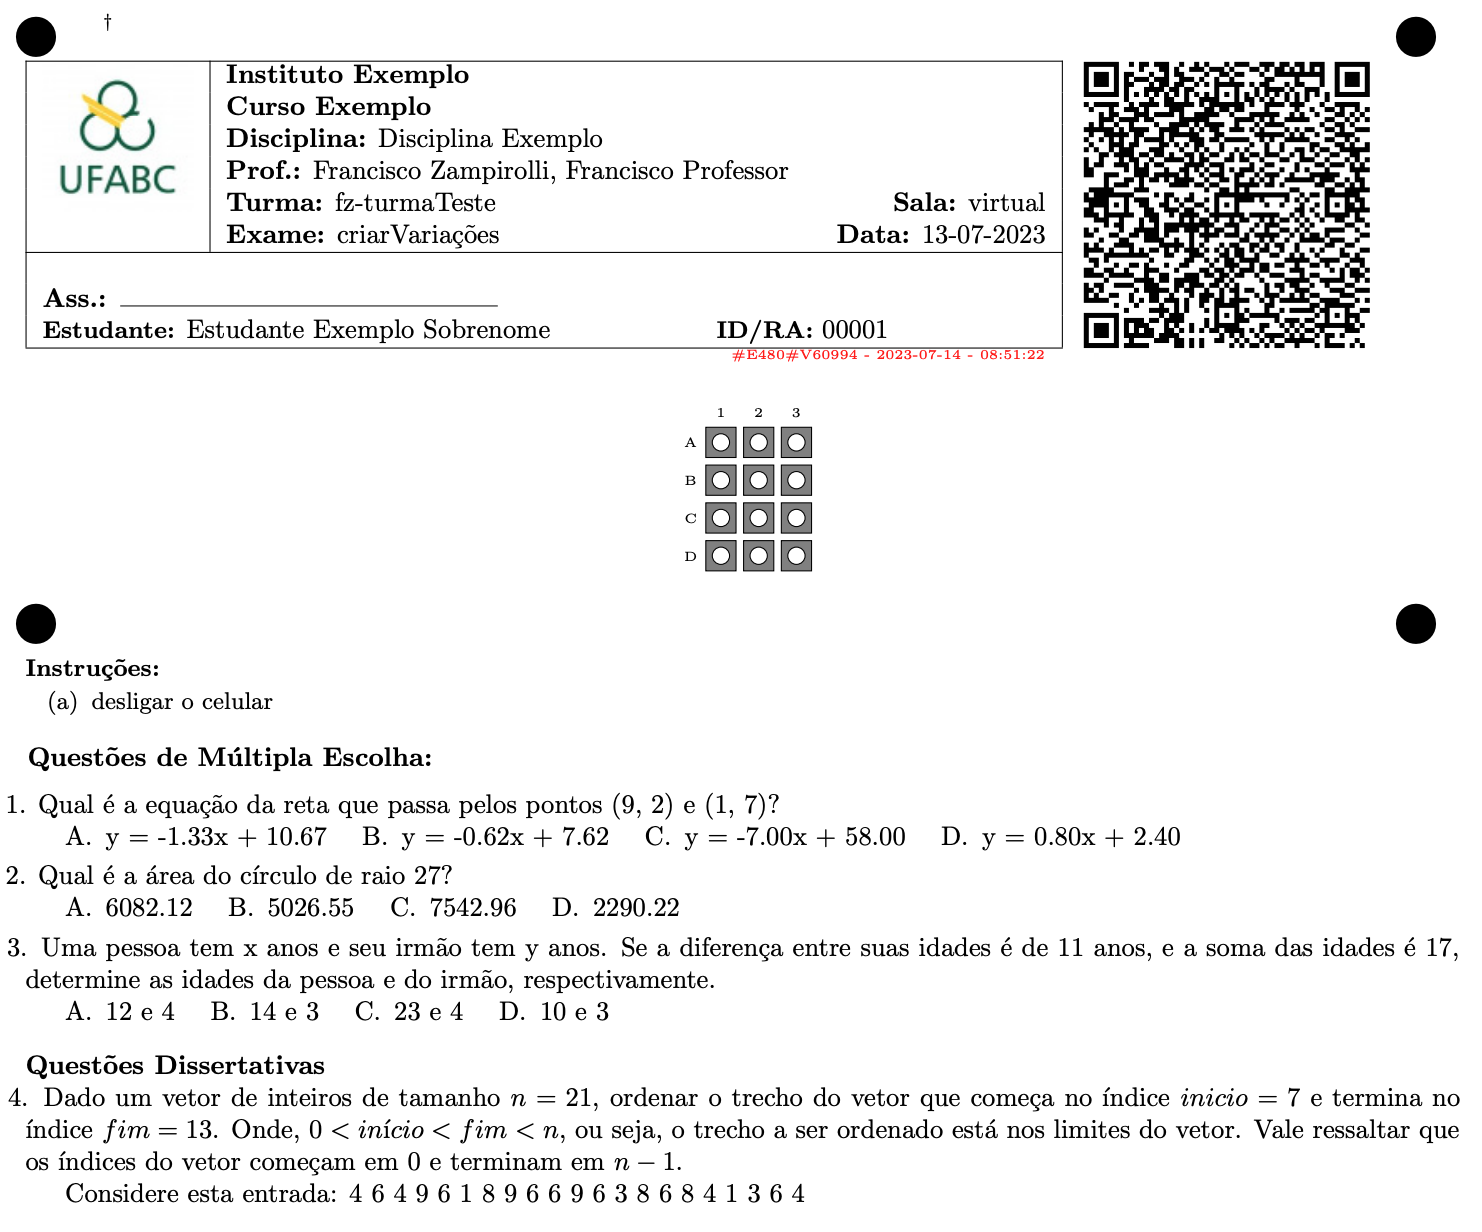
\includegraphics[width=0.9\textwidth]{cap09_exameVariacoes_PDF_MCTest.png}
  \caption{Exemplo exame gerado pelo MCTest.}
  \label{fig:cap09_exameVariacoes_PDF_MCTest}
\end{figure}

\section{Considerações finais} 

Neste capítulo apresentou-se a utilização do recurso do MCTest que permite exportar variações de um exame nos formatos Aiken e XML para o Moodle, a fim de criar um banco de questões. Utilizou-se uma questão apresentada no Capítulo \ref{ch:examesQM_QT} - \nameref{ch:examesQM_QT}, além de criar novas questões para exemplificar o processo.

Verificou-se que o uso do MCTest para criar o banco de questões é vantajoso em comparação à criação de questões parametrizadas diretamente no Moodle, uma vez que o MCTest suporta uma variedade maior de parametrizações de questões. Após configurar o exame para gerar variações, é possível exportá-las nos formatos Aiken ou XML e importá-las para o banco de questões do Moodle, criando uma atividade com as questões importadas. Dessa forma, é possível criar atividades muito mais parametrizadas do que aquelas suportadas apenas pelos valores curinga no Moodle.

Na seção de criação do exame e exportação das variações, foram demonstrados exemplos de como criar um exame com três QMs paramétricas e uma QT com resposta exata, explicando como o MCTest pode ser utilizado para gerar variações.

Foi detalhado o conteúdo dos arquivos nos formatos Aiken e XML para as QMs e QTs com respostas exatas, destacando a necessidade de remover os comentários adicionados pelo MCTest nos arquivos Aiken antes de importá-los para o Moodle. Quanto aos arquivos XML, ressaltou-se a complexidade da sintaxe e a importância de remover os comentários em \LaTeX{} dentro de cada questão no MCTest. Também foi necessário prestar atenção especial à formatação utilizada, como a matemática, já que pode ser inválida no Moodle.

Por fim, apresentou-se um tutorial para importar e criar questionários no Moodle utilizando o formato XML, mostrando como acessar a opção de importação, escolher o formato XML e carregar o arquivo correspondente. Demonstrou-se que as questões são carregadas no Moodle, mesmo que haja algumas limitações na formatação em \LaTeX{}.

Concluiu-se que o uso do MCTest em conjunto com o Moodle é uma abordagem eficaz para criar exames com uma variedade maior de questões parametrizadas, superando as limitações do Moodle na criação dessas questões. A exportação das variações nos formatos Aiken e XML permite uma integração mais fluida e flexível entre as duas plataformas, possibilitando a criação de atividades mais personalizadas e de qualidade no Moodle.

No próximo capítulo, serão abordados a criação de exames contendo questões com correção automática em atividades VPL do Moodle, apresentando exemplos e detalhando todo o processo de correção automática desses exames.